\subsection{%
  \(\epsilon\)~-НКА. Преобразование \(\epsilon\)~-НКА в НКА.%
}

\begin{definition}
  \(\epsilon\)-НКА это НКА в котором \(\epsilon \in \Sigma\), т.е. возможны
  переходы из одного состояния в другое без 'чтения' символов входной строки.
\end{definition}

\begin{definition}
  \(\epsilon\)-замыканием вершины называется множество вершин, в которое можно
  добраться из этой вершины только по \(\epsilon\)-переходам.
\end{definition}

\underline{Алгоритм}:

\begin{figure}[H]
  \centering
  
  \begin{subfigure}[b]{0.45\textwidth}
    \centering
    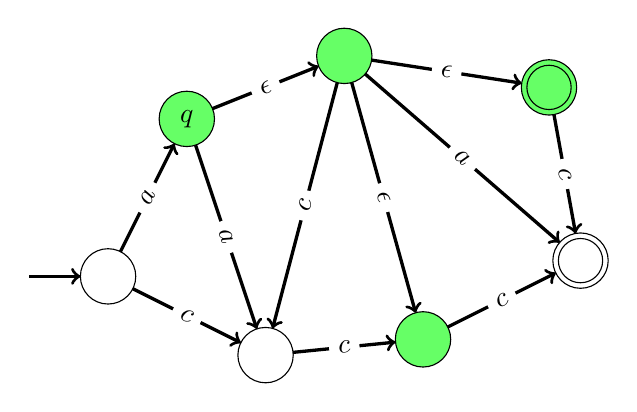
\begin{tikzpicture}[
  vertex/.style = {
    shape = circle,
    draw = black,
    minimum size = 20pt,
    inner sep = 0pt,
    outer sep = 0pt,
  }
]
  \node[vertex] (v1) at (1, 0) {};
  \node[vertex, fill = green!60] (v2) at (2, 2) {\(q\)};
  \node[vertex, fill = green!60] (v3) at (4, 2.8) {};
  \node[vertex, fill = green!60] (v4) at (6.6,  2.4) {};
  \node[vertex] (v5) at (7, 0.2) {};
  \node[vertex, fill = green!60] (v6) at (5, -0.8) {};
  \node[vertex] (v7) at (3, -1) {};

  \draw (6.6, 2.4) circle (8pt);
  \draw (7, 0.2) circle (8pt);

  \begin{scope}[
    every path/.style = {->, very thick },
    every node/.style = { midway, sloped, fill = white }
  ]
    \draw (0, 0) -- (v1);
    \draw (v1) -- (v2) node {\(a\)};
    \draw (v1) -- (v7) node {\(c\)};

    \draw (v2) -- (v3) node {\(\epsilon\)};
    \draw (v2) -- (v7) node {\(a\)};

    \draw (v3) -- (v4) node {\(\epsilon\)};
    \draw (v3) -- (v5) node {\(a\)};
    \draw (v3) -- (v6) node {\(\epsilon\)};
    \draw (v3) -- (v7) node {\(c\)};

    \draw (v4) -- (v5) node {\(c\)};

    \draw (v6) -- (v5) node {\(c\)};

    \draw (v7) -- (v6) node {\(c\)};
  \end{scope}
\end{tikzpicture}

    \caption{Шаг 1}

  \end{subfigure}
  \qquad
  \begin{subfigure}[b]{0.45\textwidth}
    \centering
    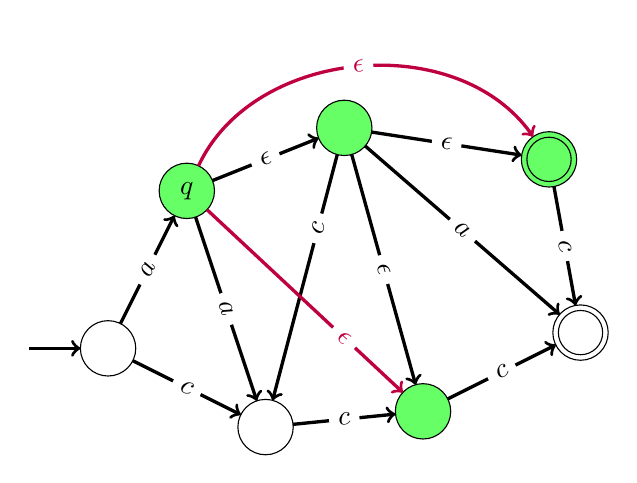
\begin{tikzpicture}[
  vertex/.style = {
    shape = circle,
    draw = black,
    minimum size = 20pt,
    inner sep = 0pt,
    outer sep = 0pt,
  }
]
  \node[vertex] (v1) at (1, 0) {};
  \node[vertex, fill = green!60] (v2) at (2, 2) {\(q\)};
  \node[vertex, fill = green!60] (v3) at (4, 2.8) {};
  \node[vertex, fill = green!60] (v4) at (6.6,  2.4) {};
  \node[vertex] (v5) at (7, 0.2) {};
  \node[vertex, fill = green!60] (v6) at (5, -0.8) {};
  \node[vertex] (v7) at (3, -1) {};

  \draw (6.6, 2.4) circle (8pt);
  \draw (7, 0.2) circle (8pt);

  \begin{scope}[
    every path/.style = {->, very thick },
    every node/.style = { midway, sloped, fill = white }
  ]
    \draw (0, 0) -- (v1);
    \draw (v1) -- (v2) node {\(a\)};
    \draw (v1) -- (v7) node {\(c\)};

    \draw (v2) -- (v3) node {\(\epsilon\)};
    \draw (v2) -- (v7) node {\(a\)};

    \draw (v3) -- (v4) node {\(\epsilon\)};
    \draw (v3) -- (v5) node {\(a\)};
    \draw (v3) -- (v6) node {\(\epsilon\)};
    \draw (v3) -- (v7) node[pos = 0.3] {\(c\)};

    \draw (v4) -- (v5) node {\(c\)};

    \draw (v6) -- (v5) node {\(c\)};

    \draw (v7) -- (v6) node {\(c\)};

    \draw[line width = 8pt, color = purple]
      (v2) edge[bend left = 60] node {\(\epsilon\)} (v4);
    \draw[line width = 8pt, color = purple]
      (v2) edge node[pos = 0.7] {\(\epsilon\)} (v6);

  \end{scope}
\end{tikzpicture}

    \caption{Шаг 2}

  \end{subfigure}
\end{figure}


\begin{figure}[H]
  \centering
  
  \begin{subfigure}[b]{0.45\textwidth}
    \centering
    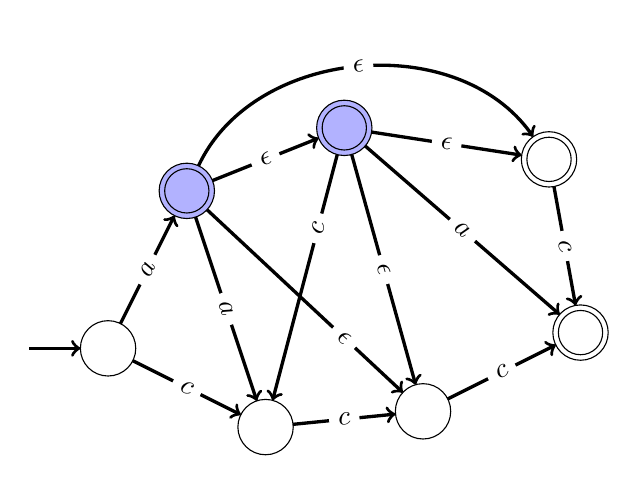
\begin{tikzpicture}[
  vertex/.style = {
    shape = circle,
    draw = black,
    minimum size = 20pt,
    inner sep = 0pt,
    outer sep = 0pt,
  }
]
  \node[vertex] (v1) at (1, 0) {};
  \node[vertex, fill = blue!30] (v2) at (2, 2) {};
  \node[vertex, fill = blue!30] (v3) at (4, 2.8) {};
  \node[vertex] (v4) at (6.6,  2.4) {};
  \node[vertex] (v5) at (7, 0.2) {};
  \node[vertex] (v6) at (5, -0.8) {};
  \node[vertex] (v7) at (3, -1) {};

  \draw (6.6, 2.4) circle (8pt);
  \draw (7, 0.2) circle (8pt);
  \draw (2, 2) circle (8pt);
  \draw (4, 2.8) circle (8pt);

  \begin{scope}[
    every path/.style = {->, very thick },
    every node/.style = { midway, sloped, fill = white }
  ]
    \draw (0, 0) -- (v1);
    \draw (v1) -- (v2) node {\(a\)};
    \draw (v1) -- (v7) node {\(c\)};

    \draw (v2) -- (v3) node {\(\epsilon\)};
    \draw (v2) -- (v7) node {\(a\)};

    \draw (v3) -- (v4) node {\(\epsilon\)};
    \draw (v3) -- (v5) node {\(a\)};
    \draw (v3) -- (v6) node {\(\epsilon\)};
    \draw (v3) -- (v7) node[pos = 0.3] {\(c\)};

    \draw (v4) -- (v5) node {\(c\)};

    \draw (v6) -- (v5) node {\(c\)};

    \draw (v7) -- (v6) node {\(c\)};

    \draw (v2) edge[bend left = 60] node {\(\epsilon\)} (v4);
    \draw (v2) edge node[pos = 0.7] {\(\epsilon\)} (v6);
  \end{scope}
\end{tikzpicture}

    \caption{Шаг 3}

  \end{subfigure}
  \qquad
  \begin{subfigure}[b]{0.45\textwidth}
    \centering
    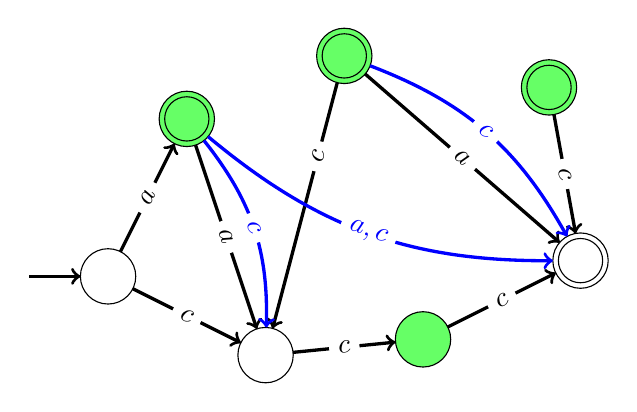
\begin{tikzpicture}[
  vertex/.style = {
    shape = circle,
    draw = black,
    minimum size = 20pt,
    inner sep = 0pt,
    outer sep = 0pt,
  }
]
  \node[vertex] (v1) at (1, 0) {};
  \node[vertex, fill = green!60] (v2) at (2, 2) {};
  \node[vertex, fill = green!60] (v3) at (4, 2.8) {};
  \node[vertex, fill = green!60] (v4) at (6.6,  2.4) {};
  \node[vertex] (v5) at (7, 0.2) {};
  \node[vertex, fill = green!60] (v6) at (5, -0.8) {};
  \node[vertex] (v7) at (3, -1) {};

  \draw (6.6, 2.4) circle (8pt);
  \draw (7, 0.2) circle (8pt);
  \draw (2, 2) circle (8pt);
  \draw (4, 2.8) circle (8pt);

  \begin{scope}[
    every path/.style = {->, very thick },
    every node/.style = { midway, sloped, fill = white }
  ]
    \draw (0, 0) -- (v1);
    \draw (v1) -- (v2) node {\(a\)};
    \draw (v1) -- (v7) node {\(c\)};

    \draw (v2) -- (v7) node {\(a\)};

    \draw (v3) -- (v5) node {\(a\)};
    \draw (v3) -- (v7) node[pos = 0.3] {\(c\)};

    \draw (v4) -- (v5) node {\(c\)};

    \draw (v6) -- (v5) node {\(c\)};

    \draw (v7) -- (v6) node {\(c\)};

    \draw[line width = 8pt, color = blue]
      (v2) edge[bend right = 20] node {\(a, c\)} (v5);
    \draw[line width = 8pt, color = blue]
      (v3) edge[bend left = 20] node {\(c\)} (v5);
    \draw[line width = 8pt, color = blue]
      (v2) edge[bend left = 20] node {\(c\)} (v7);
  \end{scope}
\end{tikzpicture}

    \caption{Шаг 4}

  \end{subfigure}
\end{figure}


\begin{enumerate}
  \item Изначальное состояние \(\epsilon\)-НКА
  
  \item Для каждого состояния \(q\) добавим \(\epsilon\)-переходы в каждое из
  состояний его \(\epsilon\)-замыкания (кроме самого состояния \(q\)).

  \item Пройдемся по всем состояниям. Если из текущего состояния есть
  \(\epsilon\)-переход в принимающее состояние, то сделаем текущее состояние
  принимающим.

  \item Для каждого перехода вида
  \(q_{1} \xrightarrow{\epsilon} q_{2} \xrightarrow{c} q_{3}\)
  добавим в НКА переход \(q_{1} \rightarrow{c} q_{3}\).
  Теперь все \(\epsilon\)-переходы можно удалить.
\end{enumerate}
